\documentclass[twoside]{book}

% Packages required by doxygen
\usepackage{fixltx2e}
\usepackage{calc}
\usepackage{doxygen}
\usepackage[export]{adjustbox} % also loads graphicx
\usepackage{graphicx}
\usepackage[utf8]{inputenc}
\usepackage{makeidx}
\usepackage{multicol}
\usepackage{multirow}
\PassOptionsToPackage{warn}{textcomp}
\usepackage{textcomp}
\usepackage[nointegrals]{wasysym}
\usepackage[table]{xcolor}

% Font selection
\usepackage[T1]{fontenc}
\usepackage[scaled=.90]{helvet}
\usepackage{courier}
\usepackage{amssymb}
\usepackage{sectsty}
\renewcommand{\familydefault}{\sfdefault}
\allsectionsfont{%
  \fontseries{bc}\selectfont%
  \color{darkgray}%
}
\renewcommand{\DoxyLabelFont}{%
  \fontseries{bc}\selectfont%
  \color{darkgray}%
}
\newcommand{\+}{\discretionary{\mbox{\scriptsize$\hookleftarrow$}}{}{}}

% Page & text layout
\usepackage{geometry}
\geometry{%
  a4paper,%
  top=2.5cm,%
  bottom=2.5cm,%
  left=2.5cm,%
  right=2.5cm%
}
\tolerance=750
\hfuzz=15pt
\hbadness=750
\setlength{\emergencystretch}{15pt}
\setlength{\parindent}{0cm}
\setlength{\parskip}{3ex plus 2ex minus 2ex}
\makeatletter
\renewcommand{\paragraph}{%
  \@startsection{paragraph}{4}{0ex}{-1.0ex}{1.0ex}{%
    \normalfont\normalsize\bfseries\SS@parafont%
  }%
}
\renewcommand{\subparagraph}{%
  \@startsection{subparagraph}{5}{0ex}{-1.0ex}{1.0ex}{%
    \normalfont\normalsize\bfseries\SS@subparafont%
  }%
}
\makeatother

% Headers & footers
\usepackage{fancyhdr}
\pagestyle{fancyplain}
\fancyhead[LE]{\fancyplain{}{\bfseries\thepage}}
\fancyhead[CE]{\fancyplain{}{}}
\fancyhead[RE]{\fancyplain{}{\bfseries\leftmark}}
\fancyhead[LO]{\fancyplain{}{\bfseries\rightmark}}
\fancyhead[CO]{\fancyplain{}{}}
\fancyhead[RO]{\fancyplain{}{\bfseries\thepage}}
\fancyfoot[LE]{\fancyplain{}{}}
\fancyfoot[CE]{\fancyplain{}{}}
\fancyfoot[RE]{\fancyplain{}{\bfseries\scriptsize Generated by Doxygen }}
\fancyfoot[LO]{\fancyplain{}{\bfseries\scriptsize Generated by Doxygen }}
\fancyfoot[CO]{\fancyplain{}{}}
\fancyfoot[RO]{\fancyplain{}{}}
\renewcommand{\footrulewidth}{0.4pt}
\renewcommand{\chaptermark}[1]{%
  \markboth{#1}{}%
}
\renewcommand{\sectionmark}[1]{%
  \markright{\thesection\ #1}%
}

% Indices & bibliography
\usepackage{natbib}
\usepackage[titles]{tocloft}
\setcounter{tocdepth}{3}
\setcounter{secnumdepth}{5}
\makeindex

% Hyperlinks (required, but should be loaded last)
\usepackage{ifpdf}
\ifpdf
  \usepackage[pdftex,pagebackref=true]{hyperref}
\else
  \usepackage[ps2pdf,pagebackref=true]{hyperref}
\fi
\hypersetup{%
  colorlinks=true,%
  linkcolor=blue,%
  citecolor=blue,%
  unicode%
}

% Custom commands
\newcommand{\clearemptydoublepage}{%
  \newpage{\pagestyle{empty}\cleardoublepage}%
}

\usepackage{caption}
\captionsetup{labelsep=space,justification=centering,font={bf},singlelinecheck=off,skip=4pt,position=top}

%===== C O N T E N T S =====

\begin{document}

% Titlepage & ToC
\hypersetup{pageanchor=false,
             bookmarksnumbered=true,
             pdfencoding=unicode
            }
\pagenumbering{alph}
\begin{titlepage}
\vspace*{7cm}
\begin{center}%
{\Large P\+ID Controller }\\
\vspace*{1cm}
{\large Generated by Doxygen 1.8.13}\\
\end{center}
\end{titlepage}
\clearemptydoublepage
\pagenumbering{roman}
\tableofcontents
\clearemptydoublepage
\pagenumbering{arabic}
\hypersetup{pageanchor=true}

%--- Begin generated contents ---
\chapter{Class Index}
\section{Class List}
Here are the classes, structs, unions and interfaces with brief descriptions\+:\begin{DoxyCompactList}
\item\contentsline{section}{\hyperlink{classPID}{P\+ID} \\*A class representing the \hyperlink{classPID}{P\+ID} controller }{\pageref{classPID}}{}
\end{DoxyCompactList}

\chapter{File Index}
\section{File List}
Here is a list of all documented files with brief descriptions\+:\begin{DoxyCompactList}
\item\contentsline{section}{include/\hyperlink{PID_8h}{P\+I\+D.\+h} \\*A header file to compute error for a \hyperlink{classPID}{P\+ID} Controller }{\pageref{PID_8h}}{}
\end{DoxyCompactList}

\chapter{Class Documentation}
\hypertarget{classPID}{}\section{P\+ID Class Reference}
\label{classPID}\index{P\+ID@{P\+ID}}


A class representing the \hyperlink{classPID}{P\+ID} controller.  




{\ttfamily \#include $<$P\+I\+D.\+h$>$}

\subsection*{Public Member Functions}
\begin{DoxyCompactItemize}
\item 
\mbox{\Hypertarget{classPID_a0311b6f7de348499ce24e53ba353514a}\label{classPID_a0311b6f7de348499ce24e53ba353514a}} 
\hyperlink{classPID_a0311b6f7de348499ce24e53ba353514a}{P\+ID} ()
\begin{DoxyCompactList}\small\item\em Construct a new \hyperlink{classPID}{P\+ID} object. Sets values of kp, ki, kd to 0. \end{DoxyCompactList}\item 
double \hyperlink{classPID_a0b9d04c13dc740eaf8f7ce408ebe2fe5}{Get\+KP} ()
\begin{DoxyCompactList}\small\item\em Returns the proportional constant. \end{DoxyCompactList}\item 
double \hyperlink{classPID_aff6252318303da61600d6d10bd16cc83}{Get\+KI} ()
\begin{DoxyCompactList}\small\item\em Returns the integral constant. \end{DoxyCompactList}\item 
double \hyperlink{classPID_ab36efdea8287d9389fa9ef83b35569b2}{Get\+KD} ()
\begin{DoxyCompactList}\small\item\em Returns the differential constant. \end{DoxyCompactList}\item 
void \hyperlink{classPID_af0770e8c485faac734274e91692ec005}{Set\+KP} (double \+\_\+kp)
\begin{DoxyCompactList}\small\item\em Updates the proportional constant attribute to \+\_\+kp. \end{DoxyCompactList}\item 
void \hyperlink{classPID_a36036f3b87f536408dad924bae81394b}{Set\+KD} (double \+\_\+kd)
\begin{DoxyCompactList}\small\item\em Updates the differential constant attribute to \+\_\+kd. \end{DoxyCompactList}\item 
void \hyperlink{classPID_af533c956b594242689fb74d758106937}{Set\+KI} (double \+\_\+ki)
\begin{DoxyCompactList}\small\item\em Updates the integral constant attribute to \+\_\+ki. \end{DoxyCompactList}\item 
double \hyperlink{classPID_ad5113ca1c4111c36945646a2f23f6a3a}{Compute\+Error} (double target\+\_\+velocity, double current\+\_\+velocity)
\begin{DoxyCompactList}\small\item\em Invokes methods to calculte P-\/\+I-\/D error \& returns the final error. \end{DoxyCompactList}\end{DoxyCompactItemize}
\subsection*{Private Member Functions}
\begin{DoxyCompactItemize}
\item 
void \hyperlink{classPID_a59aa8f314e7dad1db04cad16af197935}{Compute\+Proportional\+Error} (double target\+\_\+velocity, double current\+\_\+velocity)
\begin{DoxyCompactList}\small\item\em Computes \& sets the proportional error using the target \& current velocity of the system to the proportional\+\_\+error attribute. \end{DoxyCompactList}\item 
void \hyperlink{classPID_a4af936207ba4f04163709e4bfd909468}{Compute\+Integral\+Error} (double target\+\_\+velocity, double current\+\_\+velocity)
\begin{DoxyCompactList}\small\item\em Computes \& sets the integral error using the target \& current velocity of the system to the integral\+\_\+error attribute. \end{DoxyCompactList}\item 
void \hyperlink{classPID_a6ad839da6f331ec367d1c379960d2aa5}{Compute\+Differential\+Error} (double target\+\_\+velocity, double current\+\_\+velocity)
\begin{DoxyCompactList}\small\item\em Computes \& sets the differential error using the target \& current velocity of the system to the differential\+\_\+error attribute. \end{DoxyCompactList}\end{DoxyCompactItemize}
\subsection*{Private Attributes}
\begin{DoxyCompactItemize}
\item 
\mbox{\Hypertarget{classPID_a1d61c12e44fa9917dfc5c104493f5f29}\label{classPID_a1d61c12e44fa9917dfc5c104493f5f29}} 
double \hyperlink{classPID_a1d61c12e44fa9917dfc5c104493f5f29}{kp}
\begin{DoxyCompactList}\small\item\em Variable to store the \hyperlink{classPID}{P\+ID} proportional constant. \end{DoxyCompactList}\item 
\mbox{\Hypertarget{classPID_a750722249a34a914f6e2f05cd9d4dee3}\label{classPID_a750722249a34a914f6e2f05cd9d4dee3}} 
double \hyperlink{classPID_a750722249a34a914f6e2f05cd9d4dee3}{ki}
\begin{DoxyCompactList}\small\item\em Variable to store the \hyperlink{classPID}{P\+ID} integral constant. \end{DoxyCompactList}\item 
\mbox{\Hypertarget{classPID_a0094a774f6f64b4a1a9f93fd877c5df4}\label{classPID_a0094a774f6f64b4a1a9f93fd877c5df4}} 
double \hyperlink{classPID_a0094a774f6f64b4a1a9f93fd877c5df4}{kd}
\begin{DoxyCompactList}\small\item\em Variable to store the \hyperlink{classPID}{P\+ID} differential constant. \end{DoxyCompactList}\item 
\mbox{\Hypertarget{classPID_ac837139ae6aaf6c061124baa8b76f024}\label{classPID_ac837139ae6aaf6c061124baa8b76f024}} 
std\+::vector$<$ double $>$ \hyperlink{classPID_ac837139ae6aaf6c061124baa8b76f024}{previous\+\_\+errors}
\begin{DoxyCompactList}\small\item\em Stores all the previous errors. \end{DoxyCompactList}\item 
\mbox{\Hypertarget{classPID_a4602f44f11a5d2a7c9717bae29b27470}\label{classPID_a4602f44f11a5d2a7c9717bae29b27470}} 
double \hyperlink{classPID_a4602f44f11a5d2a7c9717bae29b27470}{time\+\_\+difference}
\begin{DoxyCompactList}\small\item\em Delta time. \end{DoxyCompactList}\item 
\mbox{\Hypertarget{classPID_a943cd212eec6928ce284f42c1d34d629}\label{classPID_a943cd212eec6928ce284f42c1d34d629}} 
double \hyperlink{classPID_a943cd212eec6928ce284f42c1d34d629}{integral\+\_\+error}
\begin{DoxyCompactList}\small\item\em Stores current integral error. \end{DoxyCompactList}\item 
\mbox{\Hypertarget{classPID_a7c8e4c28da8061d6977412d0e8a7d2f2}\label{classPID_a7c8e4c28da8061d6977412d0e8a7d2f2}} 
double \hyperlink{classPID_a7c8e4c28da8061d6977412d0e8a7d2f2}{proportional\+\_\+error}
\begin{DoxyCompactList}\small\item\em Stores current proportional error. \end{DoxyCompactList}\item 
\mbox{\Hypertarget{classPID_a40170427ce17f12276bf8abe7b107c55}\label{classPID_a40170427ce17f12276bf8abe7b107c55}} 
double \hyperlink{classPID_a40170427ce17f12276bf8abe7b107c55}{differential\+\_\+error}
\begin{DoxyCompactList}\small\item\em Stores current differential error. \end{DoxyCompactList}\end{DoxyCompactItemize}


\subsection{Detailed Description}
A class representing the \hyperlink{classPID}{P\+ID} controller. 

\subsection{Member Function Documentation}
\mbox{\Hypertarget{classPID_a6ad839da6f331ec367d1c379960d2aa5}\label{classPID_a6ad839da6f331ec367d1c379960d2aa5}} 
\index{P\+ID@{P\+ID}!Compute\+Differential\+Error@{Compute\+Differential\+Error}}
\index{Compute\+Differential\+Error@{Compute\+Differential\+Error}!P\+ID@{P\+ID}}
\subsubsection{\texorpdfstring{Compute\+Differential\+Error()}{ComputeDifferentialError()}}
{\footnotesize\ttfamily void P\+I\+D\+::\+Compute\+Differential\+Error (\begin{DoxyParamCaption}\item[{double}]{target\+\_\+velocity,  }\item[{double}]{current\+\_\+velocity }\end{DoxyParamCaption})\hspace{0.3cm}{\ttfamily [private]}}



Computes \& sets the differential error using the target \& current velocity of the system to the differential\+\_\+error attribute. 


\begin{DoxyParams}{Parameters}
{\em target\+\_\+velocity} & Target velocity of the system \\
\hline
{\em current\+\_\+velocity} & Current velocity of the system \\
\hline
\end{DoxyParams}
\mbox{\Hypertarget{classPID_ad5113ca1c4111c36945646a2f23f6a3a}\label{classPID_ad5113ca1c4111c36945646a2f23f6a3a}} 
\index{P\+ID@{P\+ID}!Compute\+Error@{Compute\+Error}}
\index{Compute\+Error@{Compute\+Error}!P\+ID@{P\+ID}}
\subsubsection{\texorpdfstring{Compute\+Error()}{ComputeError()}}
{\footnotesize\ttfamily double P\+I\+D\+::\+Compute\+Error (\begin{DoxyParamCaption}\item[{double}]{target\+\_\+velocity,  }\item[{double}]{current\+\_\+velocity }\end{DoxyParamCaption})}



Invokes methods to calculte P-\/\+I-\/D error \& returns the final error. 


\begin{DoxyParams}{Parameters}
{\em target\+\_\+velocity} & Target velocity of the system \\
\hline
{\em current\+\_\+velocity} & Current velocity of the system \\
\hline
\end{DoxyParams}
\begin{DoxyReturn}{Returns}
double Final Error 
\end{DoxyReturn}
\mbox{\Hypertarget{classPID_a4af936207ba4f04163709e4bfd909468}\label{classPID_a4af936207ba4f04163709e4bfd909468}} 
\index{P\+ID@{P\+ID}!Compute\+Integral\+Error@{Compute\+Integral\+Error}}
\index{Compute\+Integral\+Error@{Compute\+Integral\+Error}!P\+ID@{P\+ID}}
\subsubsection{\texorpdfstring{Compute\+Integral\+Error()}{ComputeIntegralError()}}
{\footnotesize\ttfamily void P\+I\+D\+::\+Compute\+Integral\+Error (\begin{DoxyParamCaption}\item[{double}]{target\+\_\+velocity,  }\item[{double}]{current\+\_\+velocity }\end{DoxyParamCaption})\hspace{0.3cm}{\ttfamily [private]}}



Computes \& sets the integral error using the target \& current velocity of the system to the integral\+\_\+error attribute. 


\begin{DoxyParams}{Parameters}
{\em target\+\_\+velocity} & Target velocity of the system \\
\hline
{\em current\+\_\+velocity} & Current velocity of the system \\
\hline
\end{DoxyParams}
\mbox{\Hypertarget{classPID_a59aa8f314e7dad1db04cad16af197935}\label{classPID_a59aa8f314e7dad1db04cad16af197935}} 
\index{P\+ID@{P\+ID}!Compute\+Proportional\+Error@{Compute\+Proportional\+Error}}
\index{Compute\+Proportional\+Error@{Compute\+Proportional\+Error}!P\+ID@{P\+ID}}
\subsubsection{\texorpdfstring{Compute\+Proportional\+Error()}{ComputeProportionalError()}}
{\footnotesize\ttfamily void P\+I\+D\+::\+Compute\+Proportional\+Error (\begin{DoxyParamCaption}\item[{double}]{target\+\_\+velocity,  }\item[{double}]{current\+\_\+velocity }\end{DoxyParamCaption})\hspace{0.3cm}{\ttfamily [private]}}



Computes \& sets the proportional error using the target \& current velocity of the system to the proportional\+\_\+error attribute. 


\begin{DoxyParams}{Parameters}
{\em target\+\_\+velocity} & Target velocity of the system \\
\hline
{\em current\+\_\+velocity} & Current velocity of the system \\
\hline
\end{DoxyParams}
\mbox{\Hypertarget{classPID_ab36efdea8287d9389fa9ef83b35569b2}\label{classPID_ab36efdea8287d9389fa9ef83b35569b2}} 
\index{P\+ID@{P\+ID}!Get\+KD@{Get\+KD}}
\index{Get\+KD@{Get\+KD}!P\+ID@{P\+ID}}
\subsubsection{\texorpdfstring{Get\+K\+D()}{GetKD()}}
{\footnotesize\ttfamily double P\+I\+D\+::\+Get\+KD (\begin{DoxyParamCaption}{ }\end{DoxyParamCaption})}



Returns the differential constant. 

\begin{DoxyReturn}{Returns}
double\+: Differential constant 
\end{DoxyReturn}
\mbox{\Hypertarget{classPID_aff6252318303da61600d6d10bd16cc83}\label{classPID_aff6252318303da61600d6d10bd16cc83}} 
\index{P\+ID@{P\+ID}!Get\+KI@{Get\+KI}}
\index{Get\+KI@{Get\+KI}!P\+ID@{P\+ID}}
\subsubsection{\texorpdfstring{Get\+K\+I()}{GetKI()}}
{\footnotesize\ttfamily double P\+I\+D\+::\+Get\+KI (\begin{DoxyParamCaption}{ }\end{DoxyParamCaption})}



Returns the integral constant. 

\begin{DoxyReturn}{Returns}
double\+: Integral constant 
\end{DoxyReturn}
\mbox{\Hypertarget{classPID_a0b9d04c13dc740eaf8f7ce408ebe2fe5}\label{classPID_a0b9d04c13dc740eaf8f7ce408ebe2fe5}} 
\index{P\+ID@{P\+ID}!Get\+KP@{Get\+KP}}
\index{Get\+KP@{Get\+KP}!P\+ID@{P\+ID}}
\subsubsection{\texorpdfstring{Get\+K\+P()}{GetKP()}}
{\footnotesize\ttfamily double P\+I\+D\+::\+Get\+KP (\begin{DoxyParamCaption}{ }\end{DoxyParamCaption})}



Returns the proportional constant. 

\begin{DoxyReturn}{Returns}
double\+: Proportional constant 
\end{DoxyReturn}
\mbox{\Hypertarget{classPID_a36036f3b87f536408dad924bae81394b}\label{classPID_a36036f3b87f536408dad924bae81394b}} 
\index{P\+ID@{P\+ID}!Set\+KD@{Set\+KD}}
\index{Set\+KD@{Set\+KD}!P\+ID@{P\+ID}}
\subsubsection{\texorpdfstring{Set\+K\+D()}{SetKD()}}
{\footnotesize\ttfamily void P\+I\+D\+::\+Set\+KD (\begin{DoxyParamCaption}\item[{double}]{\+\_\+kd }\end{DoxyParamCaption})}



Updates the differential constant attribute to \+\_\+kd. 


\begin{DoxyParams}{Parameters}
{\em \+\_\+kd} & \+: Differential constant value to be set \\
\hline
\end{DoxyParams}
\mbox{\Hypertarget{classPID_af533c956b594242689fb74d758106937}\label{classPID_af533c956b594242689fb74d758106937}} 
\index{P\+ID@{P\+ID}!Set\+KI@{Set\+KI}}
\index{Set\+KI@{Set\+KI}!P\+ID@{P\+ID}}
\subsubsection{\texorpdfstring{Set\+K\+I()}{SetKI()}}
{\footnotesize\ttfamily void P\+I\+D\+::\+Set\+KI (\begin{DoxyParamCaption}\item[{double}]{\+\_\+ki }\end{DoxyParamCaption})}



Updates the integral constant attribute to \+\_\+ki. 


\begin{DoxyParams}{Parameters}
{\em \+\_\+ki} & \+: Integral constant value to be set \\
\hline
\end{DoxyParams}
\mbox{\Hypertarget{classPID_af0770e8c485faac734274e91692ec005}\label{classPID_af0770e8c485faac734274e91692ec005}} 
\index{P\+ID@{P\+ID}!Set\+KP@{Set\+KP}}
\index{Set\+KP@{Set\+KP}!P\+ID@{P\+ID}}
\subsubsection{\texorpdfstring{Set\+K\+P()}{SetKP()}}
{\footnotesize\ttfamily void P\+I\+D\+::\+Set\+KP (\begin{DoxyParamCaption}\item[{double}]{\+\_\+kp }\end{DoxyParamCaption})}



Updates the proportional constant attribute to \+\_\+kp. 


\begin{DoxyParams}{Parameters}
{\em \+\_\+kp} & \+: Proportional constant value to be set \\
\hline
\end{DoxyParams}


The documentation for this class was generated from the following file\+:\begin{DoxyCompactItemize}
\item 
include/\hyperlink{PID_8h}{P\+I\+D.\+h}\end{DoxyCompactItemize}

\chapter{File Documentation}
\hypertarget{PID_8h}{}\section{include/\+P\+ID.h File Reference}
\label{PID_8h}\index{include/\+P\+I\+D.\+h@{include/\+P\+I\+D.\+h}}


A header file to compute error for a \hyperlink{classPID}{P\+ID} Controller.  


{\ttfamily \#include $<$vector$>$}\newline
Include dependency graph for P\+I\+D.\+h\+:
\nopagebreak
\begin{figure}[H]
\begin{center}
\leavevmode
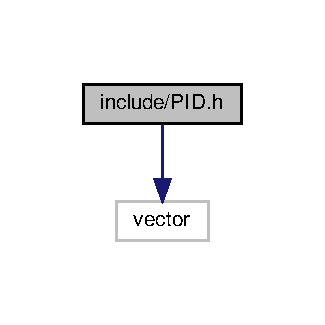
\includegraphics[width=156pt]{PID_8h__incl}
\end{center}
\end{figure}
\subsection*{Classes}
\begin{DoxyCompactItemize}
\item 
class \hyperlink{classPID}{P\+ID}
\begin{DoxyCompactList}\small\item\em A class representing the \hyperlink{classPID}{P\+ID} controller. \end{DoxyCompactList}\end{DoxyCompactItemize}


\subsection{Detailed Description}
A header file to compute error for a \hyperlink{classPID}{P\+ID} Controller. 

\begin{DoxyAuthor}{Author}
Sameer Pusegaonkar (\href{mailto:sameer@umd.edu}{\tt sameer@umd.\+edu}) -\/ Driver, Kavyashree Devadiga (\href{mailto:kavya@umd.edu}{\tt kavya@umd.\+edu}) -\/ Navigator 
\end{DoxyAuthor}
\begin{DoxyVersion}{Version}
0.\+1 
\end{DoxyVersion}
\begin{DoxyDate}{Date}
2021-\/09-\/30 
\end{DoxyDate}
\begin{DoxyCopyright}{Copyright}
Copyright (c) 2021 
\end{DoxyCopyright}

%--- End generated contents ---

% Index
\backmatter
\newpage
\phantomsection
\clearemptydoublepage
\addcontentsline{toc}{chapter}{Index}
\printindex

\end{document}
